\chapter{Experimental Results}
\label{ch:experimental-results}

\section{How to Read This Chapter}
\label{sec:results-structure}

This chapter is organized as a sequence of experiment blocks. The goal is to
make the thesis easy to navigate while many tests are still being added. Each
block follows the same structure:

\begin{enumerate}
  \item \textbf{Question.} What uncertainty or design choice does this test
  address?
  \item \textbf{Baseline and change.} Which run is the control, and what is
  changed in the comparison runs?
  \item \textbf{Protocol.} Which data split, checkpoint, seeds, and metric are
  used?
  \item \textbf{Implementation detail.} Which algorithmic, architectural, or
  mathematical change is being tested, when this is relevant?
  \item \textbf{Evidence.} Which table and figure summarize the result?
  \item \textbf{Interpretation.} What can be concluded, and what still needs to
  be verified?
\end{enumerate}

Using the same block structure for every new experiment should make it possible
to add future MSc-thesis tests without rewriting the whole results chapter.

\section{Evaluation Protocol}
\label{sec:results-evaluation-protocol}

The experiments use a train/test chronic split. The training set contains
80\% of the chronics and is used to update the policy. The test set contains
the remaining 20\% and is used to estimate generalization during training and
for final evaluation.
\\
\\
During training, evaluation rollouts are periodically run on both the train and
test splits using 10 episodes each time. In the current rerun notebook, the main
reported metric is \textbf{test episodic survival}, expressed as a percentage. 
Higher survival means that the agent keeps the grid alive for a larger fraction 
of the evaluation episodes. The final plots show seed-aggregated mean curves, 
faint individual seed curves, and the variability band.
\\
\\
The final evaluation currently uses the saved checkpoint with the best combined
train/test survival. This selection rule should be reported explicitly because
the test split participates in checkpoint selection; the values in this chapter
are therefore best interpreted as controlled rerun comparisons, not as a final
untouched test-set estimate.

\section{Experiment Index}
\label{sec:results-experiment-index}

Table~\ref{tab:experiment-index} gives a compact map of the experiment blocks
included so far. New result sections should add one row to this index before
adding detailed prose.

\begin{table}[htbp]
  \centering
  \small
  \caption{Current result blocks and their role in the thesis.}
  \label{tab:experiment-index}
  \setlength{\tabcolsep}{4pt}
  \begin{tabular}{L{0.17\textwidth}L{0.34\textwidth}L{0.32\textwidth}L{0.10\textwidth}}
    \toprule
    Block & Main question & Primary evidence & Status \\
    \midrule
    A0 core reruns & Which baseline training changes stabilize MAPPO? &
    Table~\ref{tab:a0-core-summary}, Figures~\ref{fig:rerun-a0-pairwise}
    and~\ref{fig:rerun-a0-all} & Drafted \\
    Initial do-nothing bias & Does an initial action-0 prior help exploration? &
    Table~\ref{tab:a0-bias-summary}, Figure~\ref{fig:rerun-a0-bias} & Drafted \\
    GINE reruns & Do graph encoders improve survival over the A0 baseline? &
    Tables~\ref{tab:gine-run-configurations} and~\ref{tab:gine-rerun-summary},
    Figure~\ref{fig:rerun-gine-best00} & Drafted \\
    Heavy GINE & Does a larger GINE architecture help or overcomplicate
    optimization? & Table~\ref{tab:heavy-gine-configurations},
    Figure~\ref{fig:gine-best-search2} & Drafted \\
    Sparse intervention control & Can decentralized agents intervene rarely,
    locally, and only when useful? &
    Tables~\ref{tab:sparse-control-mechanisms}
    and~\ref{tab:sparse-control-main-comparisons} & Design drafted \\
    \bottomrule
  \end{tabular}
\end{table}

\section{IEEE 14-Bus Experiments}
\label{sec:bus14-results}

The first result group focuses on the IEEE 14-bus topology-control task. The
initial PPO/MAPPO baseline from the MARL2Grid framework was not satisfactory:
the agents did not learn a robust policy and the survival rate remained low.
The following experiments therefore test training and architecture changes that
could make the baseline more stable.

\subsection{A0 Core Reruns}
\label{subsec:a0-core-reruns}

\paragraph{Question.}
Which changes are needed to obtain a stable MLP MAPPO baseline on the 14-bus
task?

\paragraph{Baseline and changes.}
The A0 family starts from the flat MLP MAPPO baseline and tests three main
stabilization choices:

\begin{itemize}
  \item increasing actor and critic capacity from two hidden layers to three
  hidden layers;
  \item using reward normalization;
  \item changing the critic update so that the critic is updated once for the
  whole batch instead of once per agent.
\end{itemize}

\paragraph{Implementation detail.}
There is no new mathematical objective in this ablation. The implementation
changes are practical training choices: network depth, reward normalization,
critic-update scheduling, and the initialization of the action-0 probability.
Table~\ref{tab:a0-run-configurations} records these settings so that the
survival plots can be interpreted without repeatedly restating the run names.

\begin{table}[htbp]
  \centering
  \scriptsize
  \caption{A0-family run configurations. The reference run is
  \texttt{rerun\_a0\_opt}.}
  \label{tab:a0-run-configurations}
  \setlength{\tabcolsep}{3pt}
  \begin{tabular}{L{0.21\textwidth}L{0.13\textwidth}L{0.10\textwidth}L{0.12\textwidth}L{0.12\textwidth}L{0.22\textwidth}}
    \toprule
    Run family & Actor/critic hidden layers & Reward norm. & Initial action-0 prob. &
    Optimized critic update & Difference from \texttt{rerun\_a0\_opt} \\
    \midrule
    \texttt{rerun\_a0\_opt} & \(3\times256\) / \(3\times256\) &
    true & 0.0 & true & Reference baseline \\
    \texttt{rerun\_a0\_nonopt} & \(3\times256\) / \(3\times256\) &
    true & 0.0 & false & Disables optimized critic updates \\
    \texttt{rerun\_a01} & \(2\times256\) / \(2\times256\) &
    true & 0.0 & true & Uses a smaller MLP actor and critic \\
    \texttt{rerun\_a02} & \(3\times256\) / \(3\times256\) &
    false & 0.0 & true & Disables reward normalization \\
    \texttt{old\_a0\_nonopt\_noval20} & \(3\times256\) / \(3\times256\) &
    true & 0.3 & false & Uses action-0 bias 0.3 and non-optimized critic updates \\
    \texttt{rerun\_bias\_05} & \(3\times256\) / \(3\times256\) &
    true & 0.5 & true & Uses action-0 bias 0.5 \\
    \texttt{rerun\_bias\_07} & \(3\times256\) / \(3\times256\) &
    true & 0.7 & true & Uses action-0 bias 0.7 \\
    \bottomrule
  \end{tabular}
\end{table}

\paragraph{Evidence.}
Table~\ref{tab:a0-core-summary} reports final and peak survival for the core A0
ablations. Figure~\ref{fig:rerun-a0-pairwise} shows each comparison against the
\texttt{rerun\_a0\_opt} baseline, and Figure~\ref{fig:rerun-a0-all} overlays all
core A0 curves.

\begin{table}[htbp]
  \centering
  \small
  \caption{A0 core rerun survival summary.}
  \label{tab:a0-core-summary}
  \resizebox{\textwidth}{!}{%
  \begin{tabular}{llrr}
    \toprule
    Run & Intended change & Final survival (\%) & Peak survival (\%) \\
    \midrule
    \texttt{rerun\_a0\_opt} & A0 optimized baseline & 93.4 & 98.6 \\
    \texttt{rerun\_a0\_nonopt} & Disable optimized critic update & 93.1 & 95.8 \\
    \texttt{rerun\_a01} & Smaller MLP actor/critic & 93.7 & 100.0 \\
    \texttt{rerun\_a02} & Disable reward normalization & 81.8 & 97.1 \\
    \texttt{old\_a0\_nonopt\_noval20} & Older non-optimized protocol & 22.3 & 68.4 \\
    \bottomrule
  \end{tabular}
  }
\end{table}

\begin{figure}[htbp]
  \centering
  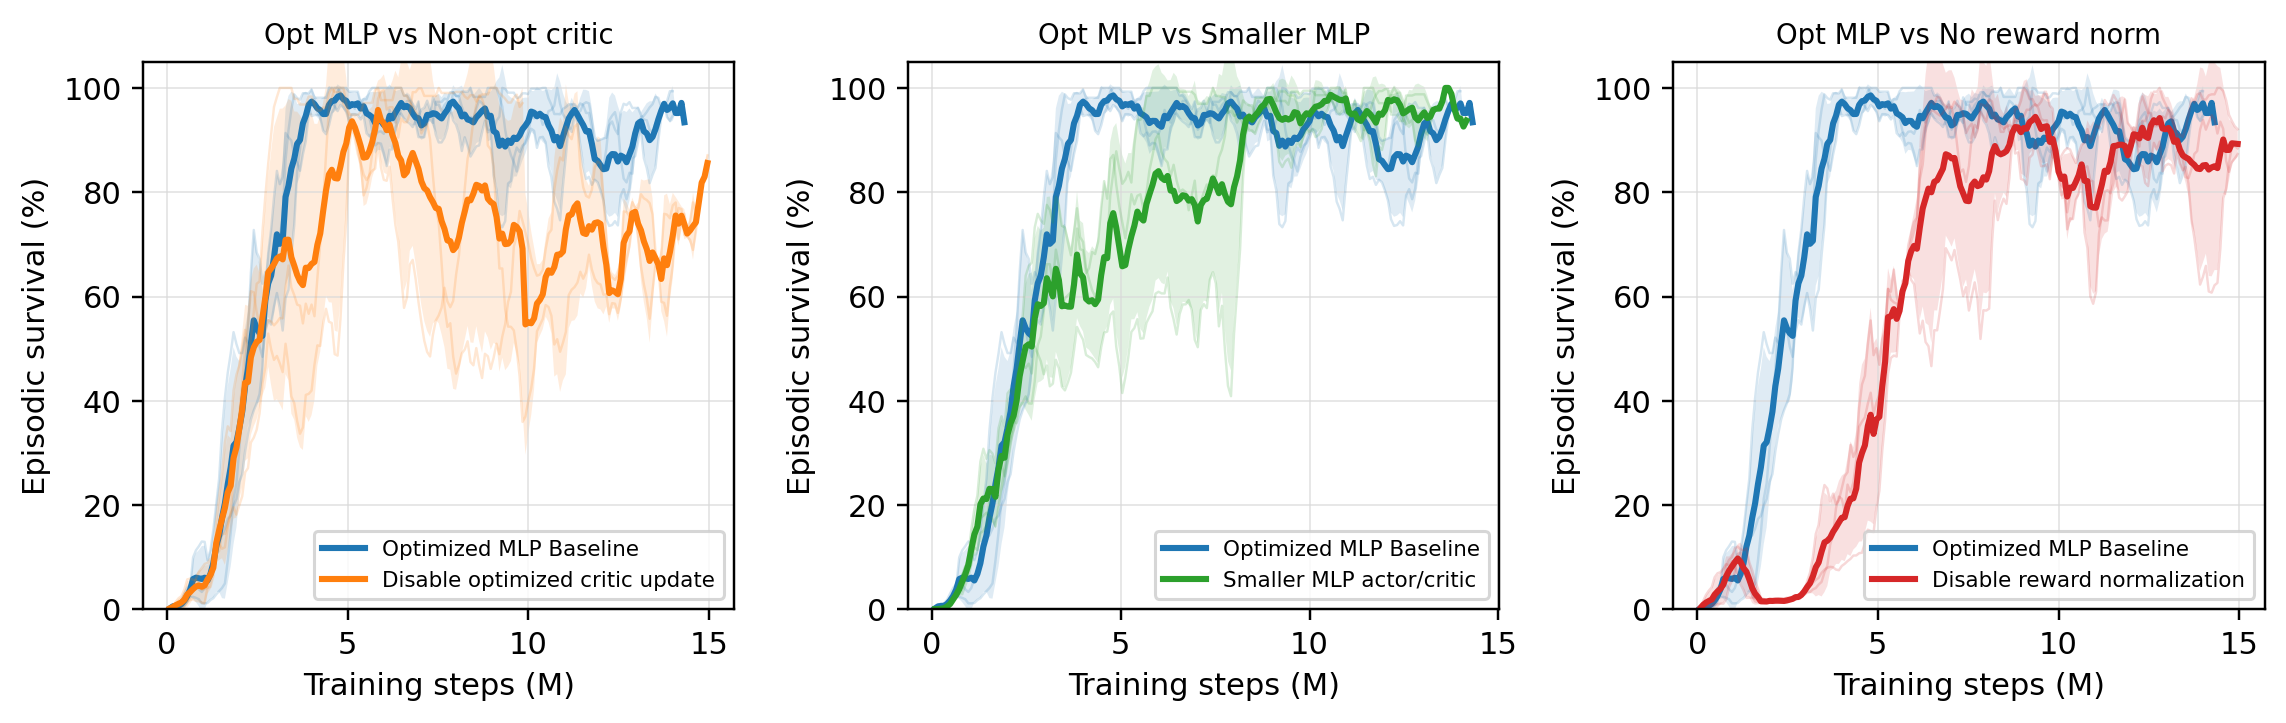
\includegraphics[width=\textwidth]{figures/rerun_a0_core_pairwise_comparisons.png}
  \caption{Pairwise A0 rerun comparisons against the \texttt{rerun\_a0\_opt}
  baseline.}
  \label{fig:rerun-a0-pairwise}
\end{figure}

\begin{figure}[htbp]
  \centering
  
\includegraphics[width=\textwidth]{figures/rerun_a0_core_all_curves.png}
  \caption{All A0 core rerun survival curves shown on one axis.}
  \label{fig:rerun-a0-all}
\end{figure}

\paragraph{Interpretation.}
The optimized A0 baseline, the non-optimized critic-update variant, and the
smaller MLP variant all finish around \(93\%\) survival. This suggests that the
main A0 recipe is robust once the rerun protocol is fixed. Disabling reward
normalization still reaches high peak survival, but it learns more slowly and
finishes lower. The old no-validation, non-optimized baseline is clearly not
competitive and should not be used as the main reference for later ablations.

\subsection{Initial Do-Nothing Bias}
\label{subsec:a0-bias-reruns}

\paragraph{Question.}
Does biasing the initial policy toward action 0, the do-nothing action, help or
hurt learning?

\paragraph{Baseline and changes.}
The A0 baseline uses no initial do-nothing bias in this rerun set. The bias
controls keep the same general protocol but change the initial probability mass
assigned to action 0.


\paragraph{Implementation detail.}
The bias is applied only at initialization: it changes the starting action
distribution before learning, without changing the reward, architecture, or PPO
objective. This makes the ablation a test of exploration bias rather than a test
of representational capacity.

\paragraph{Evidence.}
Table~\ref{tab:a0-bias-summary} and Figure~\ref{fig:rerun-a0-bias} compare the
zero-bias A0 baseline with \texttt{rerun\_bias\_05} and
\texttt{rerun\_bias\_07}.

\begin{table}[htbp]
  \centering
  \small
  \caption{Initial do-nothing bias survival summary.}
  \label{tab:a0-bias-summary}
  \begin{tabular}{lrr}
    \toprule
    Run & Final survival (\%) & Peak survival (\%) \\
    \midrule
    \texttt{rerun\_a0\_opt} & 93.4 & 98.6 \\
    \texttt{rerun\_bias\_05} & 50.8 & 70.2 \\
    \texttt{rerun\_bias\_07} & 99.3 & 100.0 \\
    \bottomrule
  \end{tabular}
\end{table}

\begin{figure}[htbp]
  \centering
  
\includegraphics[width=\textwidth]{figures/rerun_a0_bias_comparison.png}
  \caption{A0 baseline compared with initial do-nothing bias controls
  \texttt{rerun\_bias\_05} and \texttt{rerun\_bias\_07}.}
  \label{fig:rerun-a0-bias}
\end{figure}

\paragraph{Interpretation.}
The effect of the action-0 bias is large and non-monotonic. The 0.5-bias curve
remains unstable and substantially below the zero-bias baseline, whereas the
0.7-bias curve eventually reaches the highest final survival in this comparison.
The current conclusion is therefore not that larger bias is always better.
Instead, the initialization prior appears to strongly shape exploration and
should be treated as a first-order ablation variable.

\subsection{GINE Encoder Reruns}
\label{subsec:gine-reruns}

\paragraph{Question.}
Can graph encoders improve topology-control performance, and which GINE design
choices matter most?

\paragraph{Baseline and changes.}
The comparison starts from the historical \texttt{best\_00} GINE baseline. The
reruns then test lighter GINE encoders, MLP versus GNN critics, optimized critic
updates, flat-feature concatenation, A0-style entropy, and different
do-nothing-bias settings.

\paragraph{Protocol.}
All GINE runs use \texttt{gnn\_type = gine}, reward normalization,
\(15{,}000{,}000\) total timesteps, evaluation every \(80{,}000\) timesteps,
\(2{,}000\) rollout steps, deterministic evaluation, and the same 80/20 chronic
split used by the A0 experiments. The reference run is \texttt{best\_00}.

\begin{landscape}
\begin{table}[p]
  \centering
  \scriptsize
  \caption{GINE rerun configuration summary. The reference run is
  \texttt{best\_00}.}
  \label{tab:gine-run-configurations}
  \setlength{\tabcolsep}{2.4pt}
  \renewcommand{\arraystretch}{1.12}
  \begin{tabular}{L{0.095\linewidth}L{0.075\linewidth}L{0.065\linewidth}L{0.095\linewidth}L{0.050\linewidth}L{0.060\linewidth}L{0.050\linewidth}L{0.065\linewidth}L{0.070\linewidth}L{0.275\linewidth}}
    \toprule
    Run & Actor/critic encoder & GNN hidden/layers & Actor/critic heads &
    Concat flat & Edge pre-enc. & Entropy & Init action-0 & Opt. critic &
    Difference from \texttt{best\_00} \\
    \midrule
    \texttt{best\_00} & \texttt{gnn} / \texttt{gnn} & 128 / 2 &
    \(3\times256\) / \(3\times256\) & true & true & 0.02 & 0.7 & false &
    Baseline: heavy concat-flat GINE actor, GNN critic, and legacy critic updates \\
    \texttt{best\_10} & \texttt{gnn} / \texttt{mlp} & 64 / 1 &
    \(2\times128\) / \(2\times128\) & true & false & 0.02 & 0.7 & true &
    Light GINE actor, MLP critic, smaller heads, no edge pre-encoder, optimized critic updates \\
    \texttt{best\_11} & \texttt{gnn} / \texttt{gnn} & 128 / 2 &
    \(3\times256\) / \(3\times256\) & true & true & 0.02 & 0.0 & false &
    Bias ablation: same as baseline, but the initial do-nothing prior is 0.0 \\
    \texttt{best\_12} & \texttt{gnn} / \texttt{gnn} & 128 / 2 &
    \(3\times256\) / \(3\times256\) & true & true & 0.02 & 0.0 & true &
    Bias 0.0 plus optimized critic updates; otherwise heavy concat-flat GINE with GNN critic \\
    \texttt{best\_13} & \texttt{gnn} / \texttt{gnn} & 128 / 2 &
    \(3\times256\) / \(3\times256\) & true & true & 0.01 & 0.0 & true &
    A0-style heavy GINE: bias 0.0, lower entropy 0.01, optimized critic updates \\
    \texttt{best\_14} & \texttt{gnn} / \texttt{mlp} & 64 / 1 &
    \(2\times128\) / \(2\times128\) & false & false & 0.01 & 0.0 & true &
    Light A0-style GINE: MLP critic, no concat-flat, lower entropy 0.01, bias 0.0, optimized critic updates \\
    \bottomrule
  \end{tabular}
\end{table}
\end{landscape}

\paragraph{Implementation detail.}
The full GINE model architecture is described separately in
Appendix~\ref{app:gine-architecture}. This block separates representational
changes from optimization changes. The GINE encoder changes how grid
observations are embedded, while the critic type, flat-feature concatenation,
entropy setting, and critic-update schedule affect how the PPO objective is
optimized.

\paragraph{Evidence.}
Table~\ref{tab:gine-run-configurations} records the run configurations,
Table~\ref{tab:gine-rerun-summary} gives the selected survival values, and
Figure~\ref{fig:rerun-gine-best00} shows the pairwise survival curves against
\texttt{best\_00}.

\begin{table}[htbp]
  \centering
  \small
  \caption{GINE rerun survival summary.}
  \label{tab:gine-rerun-summary}
  \resizebox{\textwidth}{!}{%
  \begin{tabular}{llrr}
    \toprule
    Run & Intended change & Final survival (\%) & Peak survival (\%) \\
    \midrule
    \texttt{best\_00} & Historical GINE baseline & 59.2 & 93.9 \\
    \texttt{best\_10} & Light GINE with MLP critic & 78.9 & 90.4 \\
    \texttt{best\_12} & Optimized critic and bias 0.0 & 82.5 & 85.7 \\
    \texttt{best\_14} & Light A0-style GINE with MLP critic & 95.7 & 97.4 \\
    \bottomrule
  \end{tabular}
  }
\end{table}

\begin{figure}[htbp]
  \centering
  
\includegraphics[width=\textwidth]{figures/rerun_gine_best00_vs_best10_14.png}
  \caption{Seed-aggregated test episodic survival for GINE
  \texttt{best\_00} against \texttt{best\_10}--\texttt{best\_14}.}
  \label{fig:rerun-gine-best00}
\end{figure}

\paragraph{Interpretation.}
The strongest GINE result is \texttt{best\_14}, which reaches about
\(95.7\%\) final survival. This suggests that the graph encoder can be
competitive when it is paired with a simpler MLP critic and stable A0-style
training choices. The heavier historical GINE baseline has high peak survival
but much weaker final survival, which points to optimization stability rather
than representational capacity as the main issue.

\subsection{Heavy GINE}
\label{subsec:heavy-gine}

\paragraph{Question.}
Does the heavier concat-flat GINE baseline fail because it lacks capacity, or
because specific architectural and optimization choices make it unstable?

\paragraph{Baseline and changes.}
The reference run is \texttt{best\_00}, the historical shared-actor,
concat-flat GINE with a GNN critic and legacy critic updates. The best-search 2
family compares this baseline against controlled alternatives that change the
flat-feature concatenation, critic type, actor sharing, GNN size, entropy
schedule, node identifiers, message-passing operator, and initialization bias.

\paragraph{Protocol.}
The configurations are read from
\texttt{configs/gine\_s0\_s1\_s2}. Each family is run with seeds
\texttt{s0}, \texttt{s1}, and \texttt{s2}. Unless changed by the family, the
runs use reward normalization, deterministic evaluation, 5 evaluation episodes,
\(15{,}000{,}000\) total timesteps, evaluation every \(80{,}000\) timesteps, and
the same 80/20 chronic split.

\paragraph{Implementation detail.}
Table~\ref{tab:heavy-gine-configurations} gives the parameter comparison used
for this ablation. The table is based on the \texttt{s0} TOML file for each
family; the corresponding \texttt{s1} and \texttt{s2} files keep the same
configuration except for the training seed and run name.

\begin{landscape}
\begin{table}[p]
  \centering
  \tiny
  \caption{Heavy-GINE best-search 2 parameter comparison from
  \texttt{configs/gine\_s0\_s1\_s2}.}
  \label{tab:heavy-gine-configurations}
  \setlength{\tabcolsep}{2pt}
  \renewcommand{\arraystretch}{1.12}
  \begin{tabular}{L{0.065\linewidth}L{0.215\linewidth}L{0.045\linewidth}L{0.060\linewidth}L{0.050\linewidth}L{0.075\linewidth}L{0.045\linewidth}L{0.045\linewidth}L{0.045\linewidth}L{0.045\linewidth}L{0.060\linewidth}L{0.045\linewidth}L{0.055\linewidth}}
    \toprule
    Run & Main change from \texttt{best\_00} & GNN & GNN size & Critic &
    Actor/critic heads & Concat & Shared & Edge pre. & Node ID & Entropy &
    Init action-0 & Opt. critic \\
    \midrule
    \texttt{best\_000} & Removes flat-observation concatenation &
    \texttt{gine} & \(2\times128\) & \texttt{gnn} & \(3\times256\) / \(3\times256\) &
    no & yes & yes & yes & 0.02--0.02 & 0.7 & no \\
    \texttt{best\_00} & Reference: heavy concat-flat GINE with GNN critic &
    \texttt{gine} & \(2\times128\) & \texttt{gnn} & \(3\times256\) / \(3\times256\) &
    yes & yes & yes & yes & 0.02--0.02 & 0.7 & no \\
    \texttt{best\_01} & Enables optimized critic updates &
    \texttt{gine} & \(2\times128\) & \texttt{gnn} & \(3\times256\) / \(3\times256\) &
    yes & yes & yes & yes & 0.02--0.02 & 0.7 & yes \\
    \texttt{best\_02} & Replaces the GNN critic with an MLP critic &
    \texttt{gine} & \(2\times128\) & \texttt{mlp} & \(3\times256\) / \(3\times256\) &
    yes & yes & yes & yes & 0.02--0.02 & 0.7 & no \\
    \texttt{best\_03} & Uses non-shared actor GNN weights &
    \texttt{gine} & \(2\times128\) & \texttt{gnn} & \(3\times256\) / \(3\times256\) &
    yes & no & yes & yes & 0.02--0.02 & 0.7 & no \\
    \texttt{best\_04} & Uses a lighter GINE encoder &
    \texttt{gine} & \(1\times64\) & \texttt{gnn} & \(3\times256\) / \(3\times256\) &
    yes & yes & yes & yes & 0.02--0.02 & 0.7 & no \\
    \texttt{best\_05} & Decays entropy from 0.02 to 0.0 &
    \texttt{gine} & \(2\times128\) & \texttt{gnn} & \(3\times256\) / \(3\times256\) &
    yes & yes & yes & yes & 0.02--0.00 & 0.7 & no \\
    \texttt{best\_06} & Removes learned node-ID embeddings &
    \texttt{gine} & \(2\times128\) & \texttt{gnn} & \(3\times256\) / \(3\times256\) &
    yes & yes & yes & no & 0.02--0.02 & 0.7 & no \\
    \texttt{best\_07} & Replaces GINE with GAT message passing &
    \texttt{gat} & \(2\times128\) & \texttt{gnn} & \(3\times256\) / \(3\times256\) &
    yes & yes & yes & yes & 0.02--0.02 & 0.7 & no \\
    \texttt{best\_08} & Replaces GINE with weighted GCN message passing &
    \texttt{gcn} & \(2\times128\) & \texttt{gnn} & \(3\times256\) / \(3\times256\) &
    yes & yes & yes & yes & 0.02--0.02 & 0.7 & no \\
    \texttt{best\_09} & Light no-concat GINE with MLP critic and optimized critic updates &
    \texttt{gine} & \(1\times64\) & \texttt{mlp} & \(2\times128\) / \(2\times128\) &
    no & yes & no & yes & 0.02--0.02 & 0.7 & yes \\
    \texttt{best\_10} & Light concat-flat GINE with MLP critic and optimized critic updates &
    \texttt{gine} & \(1\times64\) & \texttt{mlp} & \(2\times128\) / \(2\times128\) &
    yes & yes & no & yes & 0.02--0.02 & 0.7 & yes \\
    \texttt{best\_11} & Removes the initial do-nothing bias &
    \texttt{gine} & \(2\times128\) & \texttt{gnn} & \(3\times256\) / \(3\times256\) &
    yes & yes & yes & yes & 0.02--0.02 & 0.0 & no \\
    \bottomrule
  \end{tabular}
\end{table}
\end{landscape}

\paragraph{Evidence.}
Figure~\ref{fig:gine-best-search2} compares the \texttt{best\_00} baseline
against each heavy-GINE alternative. Each panel shows the seed-averaged
test-survival curve for \texttt{best\_00} and one comparison family, with faint
seed curves and variability bands.

\begin{landscape}
\begin{figure}[p]
  \centering
  
\includegraphics[width=\linewidth,height=0.86\textheight,keepaspectratio]{figures/gine_best_search2_baseline_comparisons.png}
  \caption{Heavy-GINE best-search 2 survival comparisons. Each subplot compares
  the \texttt{best\_00} heavy concat-flat GINE baseline against one controlled
  alternative from \texttt{configs/gine\_s0\_s1\_s2}.}
  \label{fig:gine-best-search2}
\end{figure}
\end{landscape}

\paragraph{Interpretation.}
The broad search suggests that the heavy baseline is not limited by capacity
alone. Several simpler or more constrained variants improve final survival over
\texttt{best\_00}, especially removing node-ID embeddings, removing flat
concatenation, using an MLP critic, and combining a light GINE actor with an MLP
critic. In contrast, simply switching message passing to GAT or weighted GCN,
or removing the initial do-nothing bias while keeping the heavy GINE/GNN-critic
structure, does not clearly solve the stability problem.

\section{Decentralized Sparse Intervention Control}
\label{sec:sparse-intervention-control}

\paragraph{Question.}
Can the agents keep high survival while behaving more like operators: acting
rarely, acting locally, acting mainly when the grid state makes an intervention
useful, and keeping the final policy decentralized?

\paragraph{Baseline and change.}
This block starts from the flat decentralized MAPPO topology-control actor. For
agent \(i\), the baseline policy is one categorical distribution over the full
local action space:
\[
  \pi_i(a_i \mid o_i),
  \qquad
  a_i \in \{0,1,\ldots,|\mathcal A_i|-1\}.
\]
Action \(0\) is the no-op action. During training, actions are sampled from the
policy, while deterministic evaluation uses the greedy action by default:
\[
  a_{i,t}^{eval}=\arg\max_a \pi_i(a\mid o_{i,t}).
\]
The sparse-control roadmap tests four ways to reduce unnecessary topology
changes: evaluation-time rho overrides, an intervention-gated actor, fixed
non-idle action penalties, and adaptive Lagrangian intervention budgets.

\paragraph{Motivation.}
The intervention gate is motivated by hierarchical topology-control work, where
the action can be decomposed into ``do nothing versus intervene'', then where to
act, then which local topology configuration to apply~\cite{manczak2023hrl,
vandersar2023hmarl}. In this thesis only the first level is adapted: each
regional agent independently decides whether to do nothing or to execute one of
its existing local topology actions. The fixed and adaptive sparse-control
objectives are closer to constrained and budgeted RL: non-idle topology
interventions are treated as a limited resource, following the general
Lagrangian view of constrained policy optimization and budgeted control
\cite{achiam2017cpo,stooke2020pid,carrara2019budgeted}. This is also
operationally meaningful because switching frequency and topology deviation are
real power-grid objectives, not just cosmetic metrics~\cite{lautenbacher2025morl}.

\subsection{Evaluation-Time Rho Heuristics}
\label{subsec:sparse-control-heuristics}

\paragraph{Implementation detail.}
The rho heuristic is an evaluation-only diagnostic. It does not change the
training objective and it does not prove that the policy learned sparse
behavior. The policy first proposes the deterministic action \(\bar a_{i,t}\),
then the evaluator may replace it with action \(0\).

The global version uses the pre-action maximum line loading
\[
  \rho_t^{global}=\max_{\ell\in\mathcal L}\rho_{\ell,t},
\]
and executes
\[
  a_{i,t}^{exec}=
  \begin{cases}
    0, & \rho_t^{global}<\rho_{safe},\\
    \bar a_{i,t}, & \text{otherwise,}
  \end{cases}
  \qquad \rho_{safe}=0.90.
\]
The local version is decentralized. Agent \(i\) computes the maximum rho on the
lines touching its regional substations,
\[
  \rho_{i,t}^{local}=\max_{\ell\in\mathcal L_i}\rho_{\ell,t},
\]
and only that agent is forced to no-op when
\(\rho_{i,t}^{local}<\rho_{safe}\). A boundary line can appear in the local
neighborhood of both adjacent agents, but no communication is required: both
agents can observe the line through their own physical neighborhood.

\paragraph{Interpretation.}
The heuristic is useful to ask what happens if safe-state interventions are
blocked, but it is not a learned method. Its action-0 rates must therefore be
reported as final executed evaluation actions, not as evidence that the policy
itself prefers action \(0\).

\subsection{Intervention-Gated Actor}
\label{subsec:sparse-control-gate}

\paragraph{Implementation detail.}
The gated actor changes the actor factorization. Instead of one categorical
head over all actions, each agent has a gate head and a non-idle action head:
\[
  \pi_i^{gate}(g_i\mid o_i),\qquad g_i\in\{0,1\},
\]
where \(0\) means do nothing and \(1\) means intervene, and
\[
  \pi_i^{nonidle}(b_i\mid o_i),\qquad
  b_i\in\{1,\ldots,|\mathcal A_i|-1\}.
\]
During training, the gate is sampled first. If \(g_{i,t}=0\), then
\(a_{i,t}=0\). If \(g_{i,t}=1\), the final action is sampled from the non-idle
head. The PPO log-probability of the executed action is therefore
\[
  \log P(a_i=0)=\log P(g_i=0),
\]
and, for \(a_i>0\),
\[
  \log P(a_i)=\log P(g_i=1)+\log P(b_i=a_i\mid g_i=1).
\]

Two deterministic decoders are used. The \texttt{final\_action\_map} decoder
selects the most likely final executed action:
\[
  P(a_i=0)=P(g_i=0),\qquad
  P(a_i=a>0)=P(g_i=1)P(b_i=a\mid g_i=1).
\]
The \texttt{hierarchical\_greedy} decoder first chooses the most likely gate
decision, then chooses the most likely non-idle action only if the gate selects
intervention.

The original coupled entropy term is
\[
  H_i=H(g_i)+P(g_i=1)H(b_i).
\]
This can accidentally reward intervention because larger \(P(g_i=1)\) unlocks
more non-idle entropy. The separated entropy variant is
\[
  H_i=\alpha_{gate}H(g_i)+\alpha_{nonidle}H(b_i),
\]
and is used in the gate-plus-budget diagnostic runs.

\paragraph{Interpretation.}
The gate is learned and decentralized, but it can restrict exploration more
strongly than a reward penalty. If it collapses early to no-op, the non-idle
head is rarely executed and receives little learning signal. For this reason,
the gate is treated as an important diagnostic rather than the main sparse
control contribution.

\subsection{Fixed Sparse-Action Penalty}
\label{subsec:sparse-control-fixed-penalty}

\paragraph{Implementation detail.}
The Sparse16 sweep adds a fixed reward penalty to the final executed action of
each agent:
\[
  r'_{i,t}=r_{i,t}
  -\lambda_{fixed}\mathbf{1}[a_{i,t}\neq0],
\]
with
\[
  \lambda_{fixed}\in\{0.0,0.001,0.003,0.01\}.
\]
The grid is
\[
  \text{actor}\in\{\text{flat},\text{gated}\},\qquad
  \lambda_{fixed}\in\{0.0,0.001,0.003,0.01\},\qquad
  \text{seed}\in\{0,1,2\},
\]
which gives \(2\times4\times3=24\) runs. All Sparse16 runs set
\texttt{safe\_intervention\_penalty = 0.0}, so the penalty is not rho-weighted.

\paragraph{Interpretation.}
Sparse16 changes only the training reward. It does not override actions during
evaluation and it does not hard-mask exploration during training. The policy can
still sample non-idle actions, but each such action must be useful enough to pay
its fixed cost. The key comparison is \texttt{sparse16\_flat\_p010} versus
\texttt{sparse16\_gated\_p010}, which asks whether the gate adds value once a
simple sparse objective already exists.

\subsection{Adaptive Intervention Budget}
\label{subsec:sparse-control-aib}

\paragraph{Implementation detail.}
The adaptive intervention budget turns sparse topology control into a local
constraint. For each agent,
\[
  c_i(s_t,a_{i,t})=
  \mathbf{1}[a_{i,t}\neq0]w_i(s_t),
\]
and the desired constraint is
\[
  \mathrm{E}_{\pi_i}\left[c_i(s_t,a_{i,t})\right]\le d.
\]
The implemented rollout reward removes the constant term that does not affect
the PPO action gradient:
\[
  r'_{i,t}=r_{i,t}-\lambda_i c_i(s_t,a_{i,t}).
\]
After each rollout, the local multiplier is updated by
\[
  \lambda_i\leftarrow
  \mathrm{clip}\left(
    \lambda_i+\eta(\hat C_i-d),
    0,
    \lambda_{\max}
  \right),
  \qquad
  \hat C_i=\frac{1}{T}\sum_{t=1}^{T}c_i(s_t,a_{i,t}).
\]
If the observed cost \(\hat C_i\) is above the budget \(d\), future
interventions become more expensive; if it is below the budget, the penalty
relaxes. The default settings are \texttt{intervention\_budget\_lr = 0.02},
\texttt{intervention\_budget\_init\_lambda = 0.0}, and
\texttt{intervention\_budget\_max\_lambda = 10.0}.

Three cost modes are used:
\begin{itemize}
  \item \textbf{Non-idle cost:}
  \(w_i(s_t)=1\), so
  \(c_i(s_t,a_{i,t})=\mathbf{1}[a_{i,t}\neq0]\). This is an adaptive version
  of a plain sparse-action penalty.
  \item \textbf{Global-safe cost:}
  \(w^{global}(s_t)=\sigma(k(\rho_{safe}-\rho_t^{global}))\). This penalizes
  non-idle actions mostly when the whole grid is safe.
  \item \textbf{Local-safe cost:}
  \(w_i^{local}(s_t)=\sigma(k(\rho_{safe}-\rho_{i,t}^{local}))\). This is the
  decentralized version: safe local states make interventions expensive, while
  stressed local states make them cheap.
\end{itemize}
In the AIB setting, \(\rho_{safe}=0.90\) is not a hard action override. It is
the center of a smooth sigmoid safety weight.

\paragraph{AIB experiment grid.}
The first AIB folder, \texttt{configs/adaptive\_intervention\_budget\_7},
contains the main local-budget ablations:
\begin{itemize}
  \item \texttt{aib\_00\_flat\_local\_t020}: flat actor, local-safe cost,
  \(d=0.20\);
  \item \texttt{aib\_01\_flat\_local\_t010}: stricter local-safe budget,
  \(d=0.10\);
  \item \texttt{aib\_02\_flat\_local\_t035}: looser local-safe budget,
  \(d=0.35\);
  \item \texttt{aib\_03\_gate\_hgreedy\_sep\_local\_t020}: gated actor,
  hierarchical-greedy evaluation, separated entropy, local-safe cost,
  \(d=0.20\);
  \item \texttt{aib\_04\_flat\_nonidle\_t020}: flat actor with adaptive plain
  non-idle cost, \(d=0.20\).
\end{itemize}
The comparison \texttt{aib\_00\_flat\_local\_t020} versus
\texttt{aib\_04\_flat\_nonidle\_t020} isolates the value of local rho weighting.

The mechanism-ablation folder
\texttt{configs/adaptive\_intervention\_budget\_mechanism\_15} contains 15
additional flat-actor runs. It separates fixed versus adaptive coefficients,
plain non-idle versus state-dependent costs, global versus local rho weighting,
and rho-threshold sensitivity.

\begin{table}[htbp]
  \centering
  \small
  \caption{Sparse-control mechanisms and where they affect the policy.}
  \label{tab:sparse-control-mechanisms}
  \setlength{\tabcolsep}{3pt}
  \begin{tabular}{L{0.18\textwidth}L{0.30\textwidth}L{0.24\textwidth}L{0.18\textwidth}}
    \toprule
    Method & Training effect & Evaluation effect & Main risk \\
    \midrule
    Baseline & Samples from the flat policy & Greedy argmax by default &
    Standard entropy-controlled exploration \\
    Rho heuristic & No training change & Hard no-op override in safe states &
    Evaluation is manually changed \\
    Intervention gate & Changes action factorization and sampling &
    Final-action MAP or hierarchical greedy & Gate collapse can starve non-idle exploration \\
    Sparse16 & Fixed reward penalty on non-idle actions & No action override &
    Penalty coefficient must be tuned \\
    AIB non-idle & Adaptive reward penalty on non-idle actions & No action override &
    Multiplier can grow if target is too strict \\
    AIB local-safe & Adaptive state-dependent reward penalty & No action override &
    Depends on the local rho safety-weight design \\
    \bottomrule
  \end{tabular}
\end{table}

\begin{table}[htbp]
  \centering
  \small
  \caption{Main sparse-control comparisons to report.}
  \label{tab:sparse-control-main-comparisons}
  \setlength{\tabcolsep}{4pt}
  \begin{tabular}{L{0.45\textwidth}L{0.45\textwidth}}
    \toprule
    Question & Comparison \\
    \midrule
    Does a fixed sparse penalty already work? &
    Baseline versus \texttt{sparse16\_flat\_p010} \\
    Does the gate help beyond a sparse objective? &
    \texttt{sparse16\_flat\_p010} versus \texttt{sparse16\_gated\_p010} \\
    Fixed versus adaptive coefficient? &
    \texttt{sparse16\_flat\_p010} or \texttt{aibm\_00\_fixed\_nonidle\_p006}
    versus \texttt{aib\_04\_flat\_nonidle\_t020} \\
    Does local-safe weighting matter? &
    \texttt{aib\_00\_flat\_local\_t020} versus
    \texttt{aib\_04\_flat\_nonidle\_t020} \\
    Does global-safe weighting matter? &
    \texttt{aibm\_02\_adaptive\_global\_t020} versus
    \texttt{aib\_00\_flat\_local\_t020} \\
    Is \(\rho_{safe}=0.90\) special? &
    \texttt{aibm\_03} with \(0.85\), \texttt{aib\_00} with \(0.90\),
    and \texttt{aibm\_04} with \(0.95\) \\
    Is the heuristic only an evaluation trick? &
    Rho-heuristic runs versus learned sparse/AIB runs \\
    \bottomrule
  \end{tabular}
\end{table}

\paragraph{Metrics to report.}
The main performance metric remains episodic survival. It should be paired with
sparsity and physical-diagnostic metrics: per-agent action-0 fractions,
per-agent non-idle rates, the distribution of how many agents act
simultaneously, intervention-budget multipliers, budget costs and violations,
the rate of interventions in costly safe states, pre- and post-action max rho,
and topology-distance changes.

\paragraph{Interpretation.}
The current roadmap interpretation is that the gate is not the strongest
contribution by itself. Sparse reward shaping already improves action-0 usage,
the adaptive budget makes the sparse penalty self-tuning, and the local-safe
cost makes the penalty more physically meaningful. In particular,
\texttt{sparse16\_flat\_p010} is a strong fixed-penalty baseline, while the
most principled learned sparse-control candidate is
\texttt{aib\_00\_flat\_local\_t020}: it keeps the original decentralized actor,
does not rely on an evaluation-time override, learns the intervention penalty
adaptively, and uses a local state-dependent safety weight.

\section{Current Takeaway}
\label{sec:current-results-takeaway}

The current reruns indicate that the strongest direction is not a single
isolated modification. Stable performance comes from a combination of A0-style
training choices, reward normalization, careful initialization, and architectures
that keep the critic and graph encoder simple enough to optimize reliably.
Optimized critic updates and lighter GINE/MLP-critic variants can improve the
final GINE rerun performance, but the A0 baseline remains the clearest stable
reference point for future ablations. The sparse-control roadmap adds a second
axis to the thesis: after survival is stabilized, the next question is whether
the same decentralized agents can achieve high survival with fewer unnecessary
topology interventions.
